\documentclass{article}
\usepackage{geometry}
\geometry{a3paper, top=0.2cm, bottom=0.2cm, left=0.2cm, right=0.2cm}
\usepackage{tikz}
\usetikzlibrary{mindmap, calendar, backgrounds, shadows}
\begin{document}
\begin{center}
	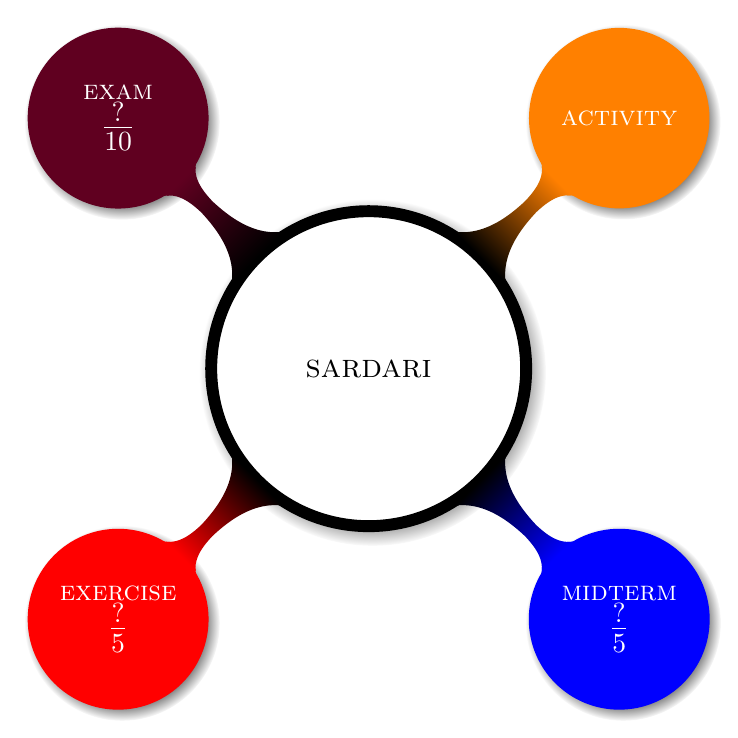
\begin{tikzpicture}[mindmap] 
		\begin{scope}[every node/.style={concept, circular drop shadow,execute at begin node=\hskip0pt},
			student/.append style={concept color=black, fill=white, line width=1ex, text=black, font=\large\scshape},
			text=white,
			exercise/.style={concept color=red,faded/.style={concept color=red!50}},
			midterm/.style={concept color=blue,faded/.style={concept color=blue!50}},
			activity/.style={concept color=orange,faded/.style={concept color=orange!50}},
			exam/.style={concept color=purple!50!black,faded/.style={concept color=green!50!black!50}},
			grow cyclic,
			level 1/.append style={level distance=4.5cm,sibling angle=90,font=\scshape},
			level 2/.append style={level distance=3cm,sibling angle=45,font=\scriptsize}]
			\node [student] {sardari}
			child [exercise] {node{exercise\\ {\Large $\frac{?}{5}$}}}
			child [midterm] {node{midterm\\ {\Large $\frac{?}{5}$}}}
			child [activity] {node{activity}}
			child [exam] {node{exam\\ {\Large $\frac{?}{10}$}}};
		\end{scope}
	\end{tikzpicture}
\end{center}
\end{document}
